\documentclass{ctexart}

\usepackage{amstext}
\usepackage{geometry}
\geometry{
  a4paper,
  total={210mm,297mm},
  left=20mm,
  right=20mm,
  top=20mm,
  bottom=20mm,
}

\usepackage{hyperref}
\hypersetup{
  bookmarksnumbered=true,
  colorlinks=true,
  allcolors=blue,
}

\usepackage[
  backend=biber,
  style=numeric,
  citestyle=ieee,
]{biblatex}
\addbibresource{translation_geometry.bib}

\usepackage{graphicx}

\usepackage{booktabs}

\usepackage{csvsimple}

\usepackage{siunitx}

\usepackage{xcolor}


\title{低矮房屋的体型对其所受龙卷风荷载影响的的研究}
\author{Jeremy Case}
\date{}

\begin{document}

\maketitle

\begin{abstract}
尽管龙卷风的破坏力巨大,但仅存在有限的尝试试图定量分析龙卷风引起的荷载。
本文的目的在于分析建筑的不同体型对其在模拟龙卷风(模拟龙卷风的涡流比根据实测龙卷风取值)作用下所受荷载和风压的影响。
测量得到的建筑所受荷载和风压被用于评估抗龙卷风设计的可行性。
龙卷风实验装置核心直径\SI{56}{m},能产生较大的涡流比(\num{2.6})以代表EF3等级龙卷风,建筑的缩尺模型放置于实验装置中,以测量其所受风压。
研究表明,最大风压与檐口高度、屋顶高度、纵横比、平面面积、及其它建筑几何形状的变化(如附加的车库、挑檐和拱腹)有关。
根据测量所得风压计算屋盖与墙、墙板与椽子的连接所需强度,并与其实际强度进行比较,以评估结构失效的概率。
结果表明,住宅中两处关键的连接(主要是屋盖与墙的连接)若设计得当,则能保证足够的安全储备以抵抗不超过EF3等级的龙卷风的袭击。
\end{abstract}

\section{引言}
许多观点质疑住宅抗龙卷风设计的可能性,遑论其可行性。
这样的观点大多来自于对结构在强风作用下的破坏程度的评估,并因龙卷风惊人的破坏力而产生偏见,
但这些观点并未依据足尺或缩尺建筑的龙卷风试验所测压力与结构构件与连接具有的实际抗力的比较。
现代工程学基于理论和经验总结的准则,但对于抗龙卷风设计,几乎没有数据能用于形成实用的工程准则。
过去,在龙卷风袭击时,屋盖所受风压及结构所受荷载的近似数据仅被用于法院的调查和工程的判断之中。
这种限制来源于三个困难:缺乏能够测量龙卷风引起的风压和荷载的仪器;缺乏实测数据与实验数据进行对比研究;
以及缺乏对抗龙卷风设计的兴趣,因为人们假定这样做是不经济的。

为了克服上文第一个困难\cite{haan2008design},爱荷华州立大学(Iowa State University, ISU)建成了一个龙卷风模拟装置。
ISU龙卷风装置能产生相对于建筑模型运动的龙卷风,也能调整多个参数以产生不同种类的龙卷风。
随着近年来几次龙卷风的实测数据的陆续发表,第二个困难也能迎刃而解了。
随后的工作比较了ISU实验室模拟的龙卷风与实测龙卷风及计算流体力学的龙卷风模型的特征。
Thampi等人的工作表明:当把低矮建筑所受ISU模拟龙卷风的风压输入到建筑的有限元模型中,相应的足尺建筑所受的破坏能够重现。
这些进步使得结构所受龙卷风荷载及风压的确定成为可能,并能据此探究经济可行的抗龙卷风设计。

本文研究了低矮建筑受到龙卷风引起的风压和荷载与建筑的几何形状及朝向的关系。
还研究了轻型木框架结构屋盖处两个最为脆弱的连接在实验室所测龙卷风风压作用下的抗掀能力,以探究抗龙卷风设计的可行性。

\section{模拟龙卷风}
只有当实验室模拟的龙卷风与实际发生的龙卷风具有相同特征时,模拟的龙卷风作用在低矮建筑上的风压才对评估抗龙卷风设计有指导意义。
为了获得结构设计所需的风压和荷载,实验室模拟的龙卷风需要具备一些关键的特征,其对结构所受荷载有着重要的影响。
根据Haan等人的研究,这些特征包括水平最大风速、龙卷风核心半径及行进轨迹、涡流比和移动速度。

\subsection{水平最大风速}
根据法院的数据,大约$90 \%$的龙卷风为F2等级或小于F2等级。
以EF(Enchanced Fujita)等级衡量,这对应着EF3等级的上界,据估计最大风速为\SI{74}{m/s}。
ASCE 7-10规范规定美国东南部和沿海地区等级II建筑的设计风速在\SI{63}{m/s}和\SI{80}{m/s}之间,
ICC规范规定相同地区的设计基本风速介于\SI{54}{m}和\SI{63}{m}。
规范规定的基本风速的范围意味着针对此风速量值进行设计是可行的。
建筑设计规范规定的设计基本风速与龙卷风的最大水平速度具有相同的量级,即\SI{74}{m/s}或更小,
选定试验模拟的龙卷风所对应的足尺龙卷风具有的水平风速为\SI{74}{m/s}。

ISU龙卷风模拟装置产生的风场在\SI{19}{mm}高度处的最大切向速度为\SI{11.6}{m/s},最大水平速度为\SI{11.7}{m/s}。
根据足尺龙卷风平均作用时间与模拟龙卷风作用时间相等的原则,
可确定最大水平风速为\SI{74}{m/s}(EF3等级)的足尺龙卷风与ISU模拟龙卷风的速度相似比为$\lambda_{\mathrm{v}}=11.7/74=1/6.3$。
根据最大切向速度归一化后的切向速度分布的等值线图见图\ref{fig:Vt-contour}。 

\begin{figure}
\centering
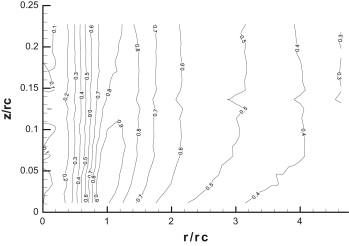
\includegraphics{./fig/1.jpg}
\caption{切向速度根据最大切向速度归一化后等值线图}
\label{fig:Vt-contour}
\end{figure}


\subsection{龙卷风核心直径}
Brooks利用报道的龙卷风破坏路径长度和宽度的数据,将藤田级数建模成Weibull分布。
根据此分布能根据具有特定藤田等级龙卷风出现的发生概率,计算其破坏路径宽度的概率。
这项研究表明,龙卷风的平均破坏宽度随藤田等级的提高而增大。
根据Brooks的结果,F1或F2等级(近似等同于EF2和EF3等级)的龙卷风,其其路径宽度近似介于\SI{100}{m}和\SI{500}{m}之间。

假定当风速达到规范规定的风速时,建筑出现破坏,对于美国中西部,设计基本风速为\SI{40}{m/s},
而EF3等级龙卷风的最大水平速度为\SI{74}{m/s},建筑的破坏可能发生在一定的范围内,这一范围可由水平风速近似超过最大切向速度的一半确定。
图\ref{fig:Vt-contour}中0.5等值线位于地表高度处大概2.2倍最大风速半径(核心半径)处。
根据Brooks的研究,EF3等级龙卷风的核心半径有很大的概率介于\SI{45}{m}和\SI{225}{m}之间。
本文的模拟龙卷风的核心半径为\SI{0.56}{m},当根据长度相似比$1:100$进行放大后,与Brooks研究得到的核心半径相符。

\subsection{涡流比}
实验室模拟龙卷风和数值模拟龙卷风最常用的参数之一是涡流比。
涡流比($S$)定义为切向动量与hexin核心半径处流量($Q$)的比值,
即$S=\pi V_{\theta \mathrm{max}}r_c^2/Q$,其中$r_c$是核心半径,
$r_c$处的切向速度为最大切向速度$V_{\theta \mathrm{max}}$。
多项研究都表明涡流比是决定龙卷风风场特征的参数。
Davies Jones展示,核心半径是涡流比的函数。
Davies Jones和Church发现涡旋的结构与涡流比相关:当涡流比增大时,涡旋分裂成多个涡旋。

足尺龙卷风的数据显示,涡流比为\num{2.0}或更大。
例如,Hangan和Kim通过比较Spencer, South Dakota发生的龙卷风与3D数值模拟龙卷风,发现涡流比最合适的设定为$S=2.0$。
根据车载多普勒雷达(DOW)测得的数据,Lee和Wurman等人计算得到,Mulhall龙卷风的涡流比介于\num{2}和\num{6}之间。
这些涡流比都是根据涡旋核心半径处($r_c$)的数据计算得到。
根据DOW测得的最新数据,并与数值模拟结果进行对比,可以发现涡流比应该增大至\num{2}或更大。
ISU龙卷风模拟装置中,产生上升气流的风口的直径为\SI{1.8}{\meter}。
气流随后直接被同心的管道引导成下降的气流。
旋转的气流通过与管道径向成一定角度的固定叶片产生。
ISU龙卷风装置可通过增大叶片角度以提高涡流比。
为了获得较大的涡流比,叶片的角度设置成\SI{75}{\degree},得到的核心半径处的涡流比为\num{2.6}。

\subsection{移动速度}
据报道,实际发生的龙卷风具有不同的移动速度:\SI{16.5}{m/s},\SI{13}{m/s}和\SI{23}{m/s}。
根据这些报道,实验室测量移动速度为\SI{0.15}{m/s}的龙卷风作用在建筑上的风压。
如果假定建筑所受破坏与其受龙卷风袭击的时间成正比,则涡旋的移动时间的相似比($\lambda_T$)应该等于$1$。
这样的设置保证了涡旋平移速度的相似比与长度的相似比一致。
因此,龙卷风装置的平移速度 \SI{1.15}{m/s}考虑到长度相似比($\lambda_L=1:100$)后,对应的足尺龙卷风的移动速度为\SI{15}{m/s}。

\subsection{地面粗糙度}
本试验用涂了清漆的胶合板模拟地面,这种胶合板很光滑。
没有引起地面粗糙的突起存在,因此可以模拟开阔平整的地面。
因为大部分的“龙卷风走廊”是乡间的农田,开阔平整的地面是合理有效的模拟对象。

\section{建筑模型,量测仪器,数据处理}
\subsection{建筑模型}
分别测量9种坡屋盖建筑模型的风压(图\ref{fig:building-models}):
不同的屋面倾角(\num{4.6}-\SI{35.5}{\degree}),屋脊高度(\num{12.2}-\SI{36}{ft}),
$L/B$比值(\num{1.0}和\num{1.5};其中$L$是长度,$B$是宽度)和
$h/L$比值(\num{0.34}-\num{0.8};其中$h$是平均屋盖高度),
是否有附属车库,并且设置多种试验工况以考虑建筑模型相对于龙卷风行进轨迹的方位角的影响。
% pressure taps
每个模型都贴有最多\num{124}个压强贴。

\begin{figure}
\centering
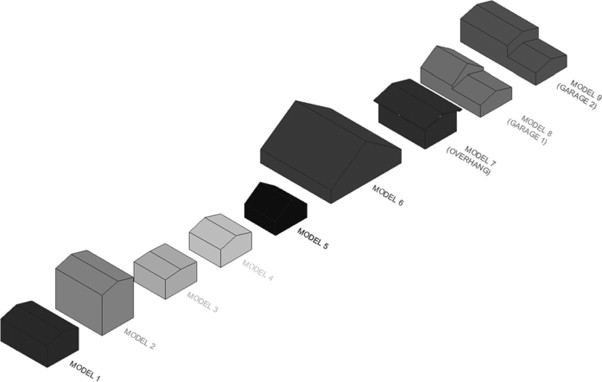
\includegraphics{./fig/2}
\caption{研究所用建筑模型}
\label{fig:building-models}
\end{figure}


模型的几何尺寸根据实际建筑尺寸经过$1:100$的相似比放大后确定,
这样才能根据试验中建筑模型的屋盖高度、纵横比、屋面倾角、挑檐距离和附加车库对模型所受模拟龙卷风的风压和荷载的影响,推测实际的情况。
模型尺寸根据常规的简易房屋设计确定,并参考ASCE 7-10规范中图6-6确定,该图将风压系数列成平均屋盖高度与建筑长度、风向和屋面倾角的比值间关系的表格。
模型尺寸列于表\ref{tab:model-dimension}。

\csvautobooktabular{./tab/table.csv}

\subsection{量测仪器}
对于静止龙卷风,采用Cobra探头(多孔探头,TFI\textregistered )测量风速,采样频率为\SI{78.1}{Hz},采样时间为\SI{26}{s}。
测点的布置间距水平向为\SI{50.8}{mm},竖向为\SI{6.35}{mm}。
测点竖向从\SI{6.35}{mm}处开始布置,直到高度为\SI{127}{mm},每竖向高度处水平布置长度为\SI{2.54}{m}。

采用两个高速64频道ZOC33/64Px压强传感器(Scanivalve Corporation\textregistered ),以\SI{390}{Hz}的采样频率测量风压。
在风压和风速量测中,仪器静压设置为实验室大气压。

\subsection{试验步骤和数据处理}
对每种工况,共测量10次风压。
对10次试验量测的风压峰值进行简单平均,作为峰值风压。
建筑模型相对于龙卷风行进路径的角度(building orientation angle,BOA)(图\ref{fig:BOA})从\SI{0}{\degree}变化到\SI{90}{\degree},角度步长为\SI{15}{\degree}。
BOA为\SI{0}{\degree}对应着龙卷风行进方向与建筑模型的屋脊平行(沿着长度 $L$方向)。
车库模型的设置角度从\SI{0}{\degree}到\SI{90}{\degree}(方位1)和\SI{180}{\degree}到\SI{270}{\degree}(方位2)。
在方位1的情况,较高的车库模型先经历龙卷风,方位2时,较低的车库模型先经历龙卷风。
所有试验工况,龙卷风的行进路径都经过建筑模型的中心。

\begin{figure}
\centering
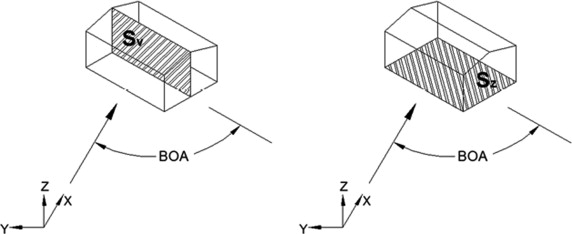
\includegraphics{./fig/3}
\caption{建筑模型相对于龙卷风行进方向轴($X$)的方位角(BOA)及用于风压系数归一化的面积($S_v$, $S_z$)}
\label{fig:BOA}
\end{figure}


风压系数沿如下方向计算:$x$向(平行于龙卷风行进方向的水平方向);$y$向(垂直于龙卷风行进方向的水平方向);$z$向(竖向)。
平面$xy$上的风ya压系数 ($C_{Fxy}$)为$x$向风压系数($C_{Fx}$)和$y$向风压系数($C_{Fy}$)平方和的根,是一个表征低矮建筑所受风荷载的重要参数。
$x$向和$y$向的风压系数利用面积$S_v$进行归一化,其中$S_v$等于屋脊高度与屋脊长度的乘积。
$z$向的风压系数利用面积$S_z$进行归一化,其中$S_z$等于建筑平面面积。
上述归一化风压系数的公式可表示为:
\begin{equation}
	C_{Fx}=\frac{F_x}{(1/2)\rho V_H^2 S_v}
\end{equation}

\begin{equation}
	C_{Fy}=\frac{F_y}{(1/2)\rho V_H^2 S_v}
\end{equation}

\begin{equation}
	C_{Fx}=\frac{F_z}{(1/2)\rho V_H^2 S_z}
\end{equation}

\begin{equation}
	C_{Fxy}=\sqrt{C_{Fx}^2+C_{Fy}^2}
\end{equation}




\printbibliography

\end{document}
